\documentclass[11pt]{article}
\usepackage[margin=1in]{geometry}
\usepackage[T1]{fontenc}
\usepackage{inconsolata}
\usepackage{enumitem}
\usepackage{hyperref}
\usepackage{xcolor}
\usepackage{forest}
\usepackage{tikz}
\usepackage{tikz-cd}
\usepackage{amsmath}
\usepackage{amssymb}

\usetikzlibrary{shapes,arrows,positioning,calc}

\hypersetup{
  colorlinks=true,
  linkcolor=blue,
  urlcolor=blue
}

\title{\textbf{Intelligent Mock Interview Agent}\\Project Structure \& Module Interaction}
\author{MockInterview.ai Hackathon Project}
\date{\today}

\begin{document}

\maketitle

\tableofcontents
\newpage

\section{Executive Summary}

The Intelligent Mock Interview Agent is a full-stack, agent-driven AI platform that automates end-to-end interview preparation. It parses resumes, infers suitable job roles, recommends matching positions, conducts adaptive mock interviews with dynamic question generation, evaluates technical answers and behavioral signals through multimodal analysis, and produces explainable feedback reports with actionable learning plans.

This document describes:
\begin{itemize}
  \item Directory structure and file organization
  \item Core agent responsibilities and services
  \item Runtime data flows and module interactions
  \item Key design patterns and architectural decisions
  \item Build, test, and deployment instructions
\end{itemize}

\newpage

\section{Repository Structure}

\subsection{Complete Directory Tree}

\begin{forest}
for tree={
  font=\ttfamily\small,
  grow'=0,
  child anchor=west,
  parent anchor=south,
  anchor=west,
  calign=first,
  edge path={
    \noexpand\path [draw, \forestoption{edge}]
    (!u.south west) +(7pt,0) |- (.child anchor)\forestoption{edge label};
  },
  before typesetting nodes={
    if n=1
      {insert before={[,phantom]}}
      {}
  },
  fit=band,
  before computing xy={l=15pt},
}
[mock-interview-agent/
  [backend/
    [agents/
      [resume\_agent.py, color=red!20]
      [role\_agent.py, color=red!20]
      [job\_recommender\_agent.py, color=red!20]
      [interview\_orchestrator.py, color=red!20]
      [intelligence\_engine.py, color=red!20]
      [evaluator\_agent.py, color=red!20]
      [feedback\_agent.py, color=red!20]
      [\_\_init\_\_.py]
    ]
    [services/
      [question\_generator.py, color=blue!20]
      [multimodal\_aggregator.py, color=blue!20]
      [audio\_analyzer.py, color=blue!20]
      [video\_analyzer.py, color=blue!20]
      [pdf\_parser.py, color=blue!20]
      [llm\_client.py, color=blue!20]
      [rubric\_service.py, color=blue!20]
      [adzuna\_job\_fetcher.py, color=blue!20]
    ]
    [routes/
      [resume\_routes.py, color=green!20]
      [role\_routes.py, color=green!20]
      [job\_routes.py, color=green!20]
      [interview\_routes.py, color=green!20]
      [scoring\_routes.py, color=green!20]
      [health.py, color=green!20]
    ]
    [models/
      [resume.py]
      [interview.py]
      [audio.py]
      [video.py]
      [analysis.py]
      [agent\_state.py]
      [jobs.py]
    ]
    [database/
      [connection.py]
      [store.py]
      [\_\_init\_\_.py]
    ]
    [tests/
      [test\_*.py]
    ]
    [config.py]
    [main.py]
    [requirements.txt]
  ]
  [frontend/
    [src/
      [pages/
        [Home.jsx]
        [ResumePage.jsx]
        [RolesPage.jsx]
        [JobsPage.jsx]
        [InterviewRoom.jsx]
        [ReportPage.jsx]
      ]
      [components/
        [AudioRecorder.jsx]
        [VideoRecorder.jsx]
        [ScoreDisplay.jsx]
        [FeedbackCharts.jsx]
        [Cards.jsx]
      ]
      [services/
        [api.js]
      ]
      [App.jsx]
      [main.jsx]
    ]
    [package.json]
    [vite.config.js]
  ]
  [docs/
    [architecture.md]
    [project\_structure.tex]
    [documentation.tex]
    [demo\_script.md]
  ]
  [sample\_data/
    [sample\_resume.txt]
    [sample\_jd.txt]
    [expected\_parsed\_resume.json]
    [expected\_roles.json]
    [expected\_job\_recommendations.json]
    [expected\_interview\_turn.json]
    [expected\_final\_report.md]
  ]
  [docker-compose.yml]
  [.env.example]
  [.dockerignore]
  [.gitignore]
  [README.md]
]
\end{forest}

\textbf{Legend:}
\begin{itemize}
  \item \colorbox{red!20}{Red}: Core agents (intelligence layer)
  \item \colorbox{blue!20}{Blue}: Services (processing \& analysis layer)
  \item \colorbox{green!20}{Green}: API routes (REST endpoints)
  \item \texttt{Routes}: FastAPI endpoint handlers
  \item \texttt{Models}: Pydantic data contracts
\end{itemize}

\newpage

\section{Backend Architecture}

\subsection{Layered Architecture}

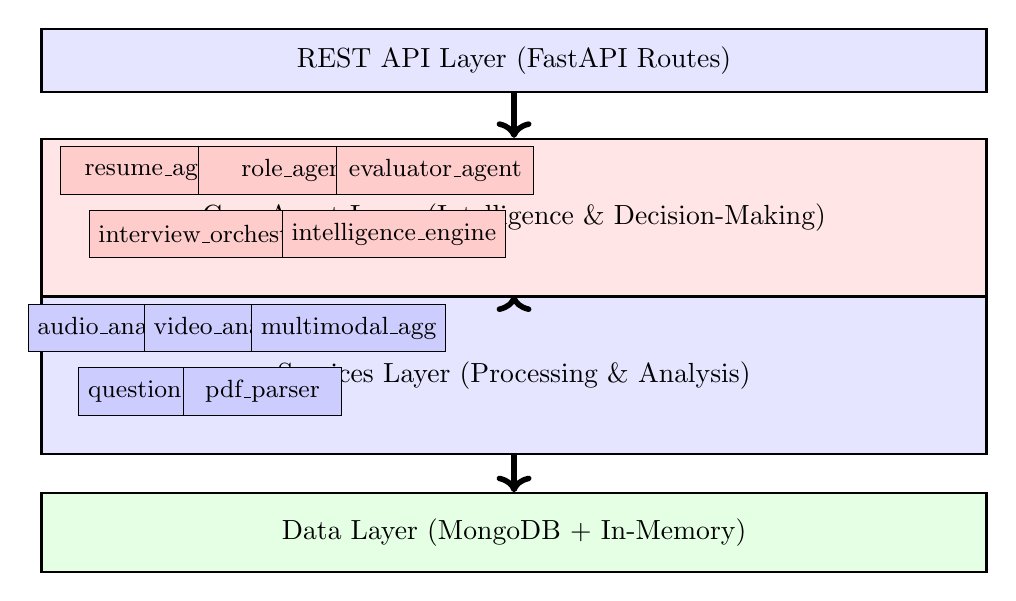
\begin{tikzpicture}[node distance=2cm, auto]
  \node[draw, thick, rectangle, minimum width=12cm, minimum height=0.8cm, fill=blue!10] (api) {REST API Layer (FastAPI Routes)};

  \node[draw, thick, rectangle, below of=api, minimum width=12cm, minimum height=2cm, fill=red!10] (agents) {Core Agent Layer (Intelligence \& Decision-Making)};

  \node[draw, thick, rectangle, below of=agents, minimum width=12cm, minimum height=2cm, fill=blue!10] (services) {Services Layer (Processing \& Analysis)};

  \node[draw, thick, rectangle, below of=services, minimum width=12cm, minimum height=1cm, fill=green!10] (data) {Data Layer (MongoDB + In-Memory)};

  \draw[->,line width=2pt] (api) -- (agents);
  \draw[->,line width=2pt] (agents) -- (services);
  \draw[->,line width=2pt] (services) -- (data);

  % Agent boxes inside
  \node[draw, rectangle, minimum width=2.5cm, minimum height=0.6cm, fill=red!20, font=\small] (agent1) at ($(agents.west) + (1.5cm, 0.6cm)$) {resume\_agent};
  \node[draw, rectangle, minimum width=2.5cm, minimum height=0.6cm, fill=red!20, font=\small] (agent2) at ($(agent1.east) + (0.5cm, 0)$) {role\_agent};
  \node[draw, rectangle, minimum width=2.5cm, minimum height=0.6cm, fill=red!20, font=\small] (agent3) at ($(agent2.east) + (0.5cm, 0)$) {evaluator\_agent};
  \node[draw, rectangle, minimum width=2.5cm, minimum height=0.6cm, fill=red!20, font=\small] (agent4) at ($(agent1.south) + (0.8cm, -0.5cm)$) {interview\_orchestrator};
  \node[draw, rectangle, minimum width=2.5cm, minimum height=0.6cm, fill=red!20, font=\small] (agent5) at ($(agent4.east) + (0.5cm, 0)$) {intelligence\_engine};

  % Service boxes inside
  \node[draw, rectangle, minimum width=2cm, minimum height=0.6cm, fill=blue!20, font=\small] (svc1) at ($(services.west) + (1cm, 0.6cm)$) {audio\_analyzer};
  \node[draw, rectangle, minimum width=2cm, minimum height=0.6cm, fill=blue!20, font=\small] (svc2) at ($(svc1.east) + (0.3cm, 0)$) {video\_analyzer};
  \node[draw, rectangle, minimum width=2cm, minimum height=0.6cm, fill=blue!20, font=\small] (svc3) at ($(svc2.east) + (0.3cm, 0)$) {multimodal\_agg};
  \node[draw, rectangle, minimum width=2cm, minimum height=0.6cm, fill=blue!20, font=\small] (svc4) at ($(svc1.south) + (0.5cm, -0.5cm)$) {question\_gen};
  \node[draw, rectangle, minimum width=2cm, minimum height=0.6cm, fill=blue!20, font=\small] (svc5) at ($(svc4.east) + (0.3cm, 0)$) {pdf\_parser};
\end{tikzpicture}

\newpage

\subsection{Core Agents}

The agent layer contains the system's core intelligence: decision-making, analysis, and evaluation.

\begin{description}[leftmargin=3cm, style=nextline]

  \item[\textbf{resume\_agent}]
  \hfill \\
  \textbf{Input}: Resume text (extracted from PDF/TXT)

  \textbf{Responsibility}: Extracts structured data from unstructured resume text.

  \textbf{Outputs}:
  \begin{itemize}
    \item Skills (technical, domain, soft)
    \item Experience (companies, roles, duration)
    \item Projects (description, technologies, impact)
    \item Education, certifications
    \item Seniority signals (years of experience, level inference)
    \item Strengths and weak areas (identified from resume gaps)
  \end{itemize}

  \textbf{Implementation}: Uses Gemini API when \texttt{USE\_LLM=true}; falls back to regex/keyword matching otherwise.

  ---

  \item[\textbf{role\_agent}]
  \hfill \\
  \textbf{Input}: Extracted resume data (skills, experience, projects)

  \textbf{Responsibility}: Ranks 8 predefined role profiles based on skill overlap and resume evidence.

  \textbf{Outputs}:
  \begin{itemize}
    \item Role recommendations (Backend, Frontend, Data, DevOps, QA, Product, ML, Embedded)
    \item Match score (0-100, Jaccard-style overlap)
    \item Matched skills and missing skills
    \item Focus areas for interview (skills to validate)
    \item Weak areas to probe (gaps in background)
    \item Project deep-dive topics
  \end{itemize}

  \textbf{Implementation}: Curated skill sets per role; Jaccard similarity for scoring.

  ---

  \item[\textbf{job\_recommender\_agent}]
  \hfill \\
  \textbf{Input}: Resume skills + selected role

  \textbf{Responsibility}: Matches candidate to live or sample job postings.

  \textbf{Outputs}:
  \begin{itemize}
    \item Top-10 ranked jobs by match score
    \item Source label (live/sample) with transparency
    \item Matched and missing skills
    \item Job details (title, company, location, salary if available)
  \end{itemize}

  \textbf{Implementation}:
  \begin{itemize}
    \item \textbf{Live}: Adzuna API (when \texttt{ADZUNA\_APP\_ID} configured)
    \item \textbf{Fallback}: 50 curated sample job listings with explicit labeling
  \end{itemize}

  ---

  \item[\textbf{interview\_orchestrator}]
  \hfill \\
  \textbf{Input}: Candidate ID, selected role

  \textbf{Responsibility}: Manages interview session state and question flow.

  \textbf{Outputs}:
  \begin{itemize}
    \item Interview session (session\_id, role, questions queue)
    \item Current question details
    \item Session progress tracking
  \end{itemize}

  \textbf{Implementation}: Maintains 5-question session; coordinates with \texttt{question\_generator} for dynamic questions.

  ---

  \item[\textbf{evaluator\_agent}]
  \hfill \\
  \textbf{Input}: Question details, candidate answer, expected concepts

  \textbf{Responsibility}: Scores technical correctness and depth of candidate responses.

  \textbf{Outputs}:
  \begin{itemize}
    \item \texttt{technical\_score} (0-100): Factual correctness
    \item \texttt{depth\_score} (0-100): Detail relative to expected points
    \item \texttt{correctness\_score} (0-100): Structure and relevance
    \item \texttt{overall\_score}: Average of above three
    \item Covered and missing concepts
    \item Improvement feedback
  \end{itemize}

  \textbf{Implementation}:
  \begin{itemize}
    \item \textbf{With Gemini}: LLM-based semantic scoring
    \item \textbf{Without Gemini}: Deterministic rubric-based scoring
  \end{itemize}

  ---

  \item[\textbf{intelligence\_engine}]
  \hfill \\
  \textbf{Input}: Technical score, audio metrics, video metrics, session history, topic coverage

  \textbf{Responsibility}: Central adaptive decision-maker. Decides next question difficulty and topic.

  \textbf{Outputs}:
  \begin{itemize}
    \item Next difficulty level (easy, medium, hard)
    \item Next topic to cover
    \item Adaptation reason (why this choice)
    \item Decision trace (for transparency)
  \end{itemize}

  \textbf{Adaptation Logic}:
  \begin{itemize}
    \item Score $< 50\%$ $\Rightarrow$ Easier next question
    \item Score $50\%-80\%$ $\Rightarrow$ Maintain difficulty
    \item Score $> 80\%$ $\Rightarrow$ Harder next question
    \item Repeated gaps $\Rightarrow$ Revisit weak areas
    \item Topic saturation $\Rightarrow$ Shift to uncovered topics
  \end{itemize}

  ---

  \item[\textbf{feedback\_agent}]
  \hfill \\
  \textbf{Input}: All interview answers, audio/video scores, technical scores, session metadata

  \textbf{Responsibility}: Generates comprehensive final report with insights and learning plan.

  \textbf{Outputs}:
  \begin{itemize}
    \item \texttt{overall\_score}: Weighted aggregate (45\% technical, 20\% communication, 15\% confidence, 10\% engagement, 10\% role-fit)
    \item Radar chart data (5 dimensions)
    \item Bar chart data (per-skill breakdown)
    \item Behavioral summary (strengths, weaknesses with evidence)
    \item Learning plan (actionable next steps)
    \item Behavioral mode label (multimodal/audio/video/fallback)
  \end{itemize}

  ---

\end{description}

\newpage

\subsection{Services}

Services handle concrete processing, analysis, and integration tasks.

\begin{description}[leftmargin=3cm, style=nextline]

  \item[\textbf{question\_generator}]
  \textbf{Service}: Dynamic interview question generation

  \textbf{Input}: Role, resume data, current difficulty, topic, previous answers

  \textbf{Output}: Question object with text, difficulty, expected concepts, rubric

  \textbf{Implementation}:
  \begin{itemize}
    \item \textbf{With Gemini}: Uses LLM to create context-aware questions
    \item \textbf{Without Gemini}: Deterministic templates grounded in role, resume, weak areas, and topic
  \end{itemize}

  ---

  \item[\textbf{audio\_analyzer}]
  \textbf{Service}: Transcription and speech analysis

  \textbf{Input}: Audio file (WAV, MP3, etc.)

  \textbf{Output}:
  \begin{itemize}
    \item Transcript (speech-to-text)
    \item \texttt{confidence\_score}: Vocal confidence (0-100)
    \item \texttt{communication\_clarity\_score}: Speech quality (0-100)
    \item Speaking rate, pause count, filler words
    \item Hesitation count and rate
    \item Metrics source label (real, fallback)
  \end{itemize}

  \textbf{Implementation}:
  \begin{itemize}
    \item \textbf{Real}: OpenAI Whisper or faster-whisper for transcription
    \item \textbf{Fallback}: File-size seeded heuristics when Whisper unavailable
  \end{itemize}

  ---

  \item[\textbf{video\_analyzer}]
  \textbf{Service}: Visual analysis and behavioral signals

  \textbf{Input}: Video frames or JPEG image

  \textbf{Output}:
  \begin{itemize}
    \item \texttt{engagement\_score}: Face detection rate (0-100)
    \item \texttt{eye\_contact\_score}: Face centering proxy (0-100)
    \item \texttt{posture\_score}: Head stability proxy (0-100)
    \item \texttt{stress\_indicator}: Inter-frame movement (low/medium/high)
    \item Frames analyzed, face detection rate
    \item Metrics source label
  \end{itemize}

  \textbf{Implementation}:
  \begin{itemize}
    \item \textbf{Real}: OpenCV + MediaPipe for face detection and landmarks
    \item \textbf{Fallback}: Reproducible random seeding for demo/dev
  \end{itemize}

  ---

  \item[\textbf{multimodal\_aggregator}]
  \textbf{Service}: Combine all scoring signals

  \textbf{Input}: Technical score, audio metrics, video metrics, role fit

  \textbf{Output}: Aggregated scores using weighted formula:
  \begin{equation}
  \text{Overall} = 0.45 \times \text{Technical} + 0.20 \times \text{Communication}
  + 0.15 \times \text{Confidence} + 0.10 \times \text{Engagement} + 0.10 \times \text{Role\text{-}Fit}
  \end{equation}

  ---

  \item[\textbf{pdf\_parser}]
  \textbf{Service}: Extract text from PDF files

  \textbf{Implementation}: PyMuPDF library for fast, reliable PDF parsing.

  ---

  \item[\textbf{llm\_client}]
  \textbf{Service}: Wrapper for Gemini API

  \textbf{Responsibility}: Handles API calls, retries, fallbacks when LLM unavailable.

  ---

  \item[\textbf{rubric\_service}]
  \textbf{Service}: Deterministic answer evaluation

  \textbf{Responsibility}: Scores answers using rule-based rubrics when Gemini API is unavailable.

  ---

  \item[\textbf{adzuna\_job\_fetcher}]
  \textbf{Service}: Live job API integration

  \textbf{Responsibility}: Fetches real job postings when credentials available; provides sample jobs otherwise.

  ---

\end{description}

\newpage

\section{Data Flow Diagrams}

\subsection{Resume Upload \& Analysis Flow}

\begin{verbatim}
User uploads PDF/TXT via Frontend
          │
          ▼
POST /api/resume/upload
          │
          ▼
pdf_parser.extract_text()  ──────►  Resume text
          │
          ▼
resume_agent.analyse(text)  ─────────┐
          │                          │
          ├─►  Uses Gemini API       │  (if USE_LLM=true)
          │    or Regex/Keywords     │  (fallback)
          │                          │
          └──────────────────────────┘
          │
          ▼
ResumeAnalysis {
  skills: [...]
  experience: [...]
  projects: [...]
  weak_areas: [...]
  strengths: [...]
  seniority: int
}
          │
          ├──► Store in MongoDB/Memory
          │
          └──► Return candidate_id + preview
\end{verbatim}

\subsection{Role \& Job Recommendation Flow}

\begin{verbatim}
GET /api/resume/roles/{candidate_id}
          │
          ▼
Fetch ResumeAnalysis by candidate_id
          │
          ▼
role_agent.recommend(resume_data)
          │
          ├─► Compute skill overlap (Jaccard similarity)
          │    for each of 8 role profiles
          │
          ├─► Identify matched/missing skills
          │
          ├─► Extract focus areas from role definition
          │
          ├─► Extract weak areas to probe
          │
          └─► Rank roles by match score
          │
          ▼
Return [{role_name, score, matched_skills, ...}] top-5
          │
          ├──► Store recommendations
          │
          └──► Frontend displays role selection UI


GET /api/jobs/{candidate_id}?role={selected_role}
          │
          ▼
job_recommender_agent.recommend(resume_data, role)
          │
          ├─► If ADZUNA_APP_ID configured:
          │    └─► adzuna_job_fetcher.fetch_live_jobs()
          │        └─► Live postings API call
          │
          ├─► Else:
          │    └─► Load 50 curated sample jobs
          │
          ├─► Match candidate skills against each job
          │
          ├─► Compute match score per job
          │
          ├─► Rank by match score
          │
          └─► Label each job as "live" or "sample"
          │
          ▼
Return [{job, score, matched_skills, source_label, ...}] top-10
\end{verbatim}

\subsection{Interview Session Flow}

\begin{verbatim}
POST /api/interview/start
          │
          ├─► candidate_id: str
          └─► selected_role: str
          │
          ▼
interview_orchestrator.start_session(candidate_id, role)
          │
          ├─► Generate session_id
          │
          ├─► Fetch ResumeAnalysis + RoleRecommendation
          │
          ├─► Initialize 5-question queue
          │
          └─► Call question_generator for first question
          │
          ▼
Question 1 returned to Frontend


User answers (typed + optional audio/video)
          │
          ▼
POST /api/interview/evaluate-answer
          │
          ├─► Answer text
          ├─► Question details
          └─► Expected concepts
          │
          ▼
evaluator_agent.evaluate(question, answer, expected_points)
          │
          ├─► Uses Gemini (if enabled)
          │    or rubric_service (fallback)
          │
          └─►  Produces: technical_score, depth_score,
                correctness_score, covered/missing points


Parallel: Audio & Video Analysis
POST /api/scoring/audio  ──► audio_analyzer  ──► confidence, clarity, pace, etc.
POST /api/scoring/video  ──► video_analyzer  ──► engagement, stress, etc.


All scores combined
          │
          ▼
multimodal_aggregator.aggregate(
  technical_score,
  communication_clarity,
  confidence,
  engagement,
  role_fit
)
          │
          ▼
overall_turn_score = weighted aggregate


Adaptation Decision
          │
          ▼
intelligence_engine.decide(
  overall_turn_score,
  audio_metrics,
  video_metrics,
  session_history,
  topic_coverage
)
          │
          ├─► If score < 50%  ──► next_difficulty = easier
          ├─► If score 50-80% ──► next_difficulty = same
          └─► If score > 80%  ──► next_difficulty = harder
          │
          ├─► Check topic coverage  ──► next_topic
          │
          └─► Store decision_trace (why this choice)
          │
          ▼
POST /api/interview/next-question
          │
          ▼
question_generator.generate(
  role,
  resume_data,
  next_difficulty,
  next_topic
)
          │
          ▼
Question 2 returned
(Repeat for questions 3-5)


After 5 questions:
POST /api/interview/final-report
          │
          ▼
feedback_agent.generate_report(session_id)
          │
          ├─► Fetch all answers + scores
          ├─► Fetch all audio/video metrics
          ├─► Compute behavioral mode
          │
          ├─► Aggregate scores per dimension
          │
          ├─► Compute overall score (45/20/15/10/10 weights)
          │
          ├─► Generate radar chart data
          ├─► Generate bar chart data
          │
          ├─► Identify strengths + evidence
          ├─► Identify weaknesses + evidence
          │
          ├─► Build learning plan
          │
          └─► Determine behavioral mode label
          │    (multimodal/audio/video/fallback/placeholder)
          │
          ▼
FinalReport returned to Frontend
Frontend renders: Radar + Bar charts, summary, learning plan
\end{verbatim}

\newpage

\section{Module Interaction Matrix}

\subsection{Agent Dependencies}

\begin{center}
\begin{tabular}{|l|c|c|c|c|c|c|c|}
\hline
\textbf{Agent} & \textbf{Resume} & \textbf{Role} & \textbf{Job} & \textbf{Orch} & \textbf{Eval} & \textbf{Intel} & \textbf{Feedback} \\
\hline
\textbf{resume\_agent} & \texttt{-} & ✓ & ✓ & ✓ & & ✓ & ✓ \\
\hline
\textbf{role\_agent} & Requires & \texttt{-} & ✓ & ✓ & & & \\
\hline
\textbf{job\_recommender} & Requires & Uses & \texttt{-} & & & & \\
\hline
\textbf{interview\_orch} & Uses & Uses & & \texttt{-} & Calls & Calls & \\
\hline
\textbf{evaluator} & & & & Calls & \texttt{-} & Uses & Uses \\
\hline
\textbf{intelligence\_eng} & Uses & Uses & & Calls & Uses & \texttt{-} & Uses \\
\hline
\textbf{feedback} & Uses & & & & Uses & Uses & \texttt{-} \\
\hline
\end{tabular}
\end{center}

\subsection{Service Dependencies}

\begin{center}
\begin{tabular}{|l|c|c|c|c|c|c|c|}
\hline
\textbf{Service} & \textbf{PDF} & \textbf{QGen} & \textbf{Audio} & \textbf{Video} & \textbf{Agg} & \textbf{LLM} & \textbf{Rubric} \\
\hline
\textbf{pdf\_parser} & \texttt{-} & & & & & & \\
\hline
\textbf{question\_gen} & & \texttt{-} & & & & Uses & Uses (fallback) \\
\hline
\textbf{audio\_analyzer} & & & \texttt{-} & & Uses & & \\
\hline
\textbf{video\_analyzer} & & & & \texttt{-} & Uses & & \\
\hline
\textbf{multimodal\_agg} & & & Uses & Uses & \texttt{-} & & \\
\hline
\textbf{llm\_client} & & Uses & & & & \texttt{-} & \\
\hline
\textbf{rubric\_service} & & Uses & & & & & \texttt{-} \\
\hline
\end{tabular}
\end{center}

\newpage

\section{API Routes \& Endpoints}

\subsection{Resume Management}

\begin{verbatim}
POST /api/resume/upload
  Multipart form-data: { file: PDF|TXT }
  Returns: { candidate_id, filename, text_preview, word_count }
  Handler: resume_routes.py

POST /api/resume/analyse
  JSON: { candidate_id: str, text: str }
  Returns: ResumeAnalysis { skills, experience, projects, ... }
  Handler: resume_routes.py
\end{verbatim}

\subsection{Role Inference}

\begin{verbatim}
GET /api/resume/roles/{candidate_id}
  Returns: { candidate_id, roles: [...] }
  Handler: role_routes.py
\end{verbatim}

\subsection{Job Discovery}

\begin{verbatim}
GET /api/jobs/{candidate_id}?role={role_name}
  Returns: { candidate_id, jobs: [...] }
  Handler: job_routes.py
\end{verbatim}

\subsection{Interview Management}

\begin{verbatim}
POST /api/interview/start
  JSON: { candidate_id, selected_role }
  Returns: { session_id, question: {...}, question_number: 1 }
  Handler: interview_routes.py

POST /api/interview/evaluate-answer
  JSON: { session_id, question_id, answer, expected_points: [...] }
  Returns: { technical_score, depth_score, correctness_score, ... }
  Handler: interview_routes.py

POST /api/interview/next-question
  JSON: { session_id, last_answer_score, confidence_score }
  Returns: { question: {...}, is_complete: bool, adaptation_reason }
  Handler: interview_routes.py

POST /api/interview/final-report
  JSON: { session_id }
  Returns: FinalReport { overall_score, radar_data, bar_data, ... }
  Handler: interview_routes.py
\end{verbatim}

\subsection{Scoring Analysis}

\begin{verbatim}
POST /api/scoring/audio
  Multipart form-data: { audio: Blob, session_id?: str }
  Returns: AudioAnalysisResponse { transcript, confidence, clarity, ... }
  Handler: scoring_routes.py

POST /api/scoring/video
  Multipart form-data: { video: Blob|JPEG, session_id?: str }
  Returns: VideoAnalysisResponse { engagement, eye_contact, stress, ... }
  Handler: scoring_routes.py
\end{verbatim}

\subsection{Health Check}

\begin{verbatim}
GET /api/health
  Returns: { status: "ok", timestamp: ISO8601 }
  Handler: health.py
\end{verbatim}

\newpage

\section{Build, Test \& Deployment}

\subsection{Quick Start}

\begin{verbatim}
# Clone and navigate
git clone <repo>
cd mock-interview-agent

# Copy environment
copy .env.example .env

# Docker Compose (full stack)
docker compose up --build

# Or background
docker compose up --build -d

# Stop
docker compose down
\end{verbatim}

Open:
\begin{itemize}
  \item Frontend: \url{http://localhost:5173}
  \item Backend Swagger: \url{http://localhost:8000/docs}
\end{itemize}

\subsection{Local Development}

\begin{verbatim}
# Backend
cd backend
python -m venv venv
.\venv\Scripts\activate
pip install -r requirements.txt
uvicorn main:app --reload --port 8000

# Frontend (new terminal)
cd frontend
npm install
npm run dev
\end{verbatim}

\subsection{Testing}

\begin{verbatim}
# Backend tests
.\venv\Scripts\python.exe -B -m pytest backend\tests

# Frontend build
cd frontend
npm run build
\end{verbatim}

\subsection{Cloud Deployment}

\begin{enumerate}
  \item Provision Docker on cloud VM
  \item Clone repository
  \item Create \texttt{.env} from \texttt{.env.example}
  \item Set \texttt{FRONTEND\_URL} and \texttt{VITE\_API\_BASE\_URL}
  \item Run: \texttt{docker compose up --build -d}
  \item For production: Use managed MongoDB, HTTPS, secret storage
\end{enumerate}

\newpage

\section{Sample Data \& Evaluation}

\subsection{Quick Evaluation Checklist}

\begin{enumerate}
  \item \textbf{Start Platform}: \texttt{docker compose up --build}
  \item \textbf{Upload Resume}: Use \texttt{sample\_data/sample\_resume.txt}
  \item \textbf{Verify Parsing}: Compare with \texttt{expected\_parsed\_resume.json}
  \item \textbf{Check Roles}: Verify output matches \texttt{expected\_roles.json}
  \item \textbf{Review Jobs}: Check for live/sample badges
  \item \textbf{Conduct Interview}: Answer 1-2 questions with audio/video
  \item \textbf{Review Scores}: Check technical + audio/video breakdowns
  \item \textbf{Generate Report}: Compare final output structure with \texttt{expected\_final\_report.md}
\end{enumerate}

\subsection{Sample Files}

\begin{tabular}{|l|p{8cm}|}
\hline
\textbf{File} & \textbf{Purpose} \\
\hline
\texttt{sample\_resume.txt} & Example resume for testing resume parser \\
\hline
\texttt{expected\_parsed\_resume.json} & Expected output from resume\_agent \\
\hline
\texttt{expected\_roles.json} & Expected role recommendations \\
\hline
\texttt{expected\_job\_recommendations.json} & Expected job matches \\
\hline
\texttt{expected\_interview\_turn.json} & Sample interview turn with scores \\
\hline
\texttt{expected\_final\_report.md} & Sample final feedback report \\
\hline
\end{tabular}

\newpage

\section{Key Design Decisions}

\subsection{Table of Trade-offs}

\begin{center}
\begin{tabular}{|l|p{4cm}|p{4cm}|p{3cm}|}
\hline
\textbf{Decision} & \textbf{Rationale} & \textbf{Trade-off} & \textbf{When to Change} \\
\hline
In-memory fallback & Zero-setup demo; no DB required & Data lost on restart; not multi-user & Production: use managed MongoDB \\
\hline
Rule-based + LLM dual mode & Works without API key & Less nuanced without LLM & Production: require API key \\
\hline
Whisper for audio & State-of-the-art; open-source & Large ~1GB; slow first load & Fast setup: use Google Cloud Speech \\
\hline
OpenCV + MediaPipe & No cloud API needed & Lower accuracy; heavy deps & Production: use cloud vision API \\
\hline
5-question sessions & Manageable interview flow & Shallow coverage per session & Deep assessment: 10+ questions \\
\hline
candidate\_id in localStorage & Simple; no auth needed & Single-device; no persistence & Production: add JWT + accounts \\
\hline
Threshold-based adaptation & Simple logic; transparent & Not IRT model; less optimal & Research: implement IRT model \\
\hline
\end{tabular}
\end{center}

\section{Known Limitations}

\begin{itemize}
  \item \textbf{No Authentication}: Designed for hackathon demo; add JWT for production
  \item \textbf{50 Static Jobs}: Not live job board; Adzuna API provides fresh listings
  \item \textbf{5 Questions}: Deeper coverage needs follow-up sessions or longer interviews
  \item \textbf{Audio Fallback}: File-size heuristics without Whisper; real analysis when available
  \item \textbf{Video Fallback}: Reproducible random numbers without OpenCV; transparency labels all modes
  \item \textbf{Eye Contact}: Face-centering proxy; not true gaze estimation
  \item \textbf{Single-Turn Evaluation}: Each answer scored independently; no cross-question context
  \item \textbf{English-Only}: Prompts and evaluators are English-only
\end{itemize}

\newpage

\section{Conclusion}

The Intelligent Mock Interview Agent uses a layered, agent-driven architecture to provide end-to-end interview preparation. The separation of agents (intelligence), services (processing), and routes (API) allows clear responsibilities, easy testing, and flexible configuration for demo, local, and cloud deployments.

Key strengths:
\begin{itemize}
  \item \textbf{Modular}: Each agent handles one concern; services are reusable
  \item \textbf{Transparent}: Decision traces, mode labels, and fallback handling are explicit
  \item \textbf{Adaptive}: Real-time difficulty adjustment based on multimodal signals
  \item \textbf{Flexible}: Works without APIs (deterministic fallbacks); improved with APIs (Gemini, Adzuna, Whisper)
  \item \textbf{Scalable}: Docker-ready; in-memory fallback for quick demos; MongoDB for production
\end{itemize}

For more details, see \texttt{docs/architecture.md} and \texttt{docs/documentation.tex}.

\end{document}
